
% =========================
% Orientações Gerais do Modelo de Slides
% =========================
% 
% Autor: Bruno Francisco Schaden
% Curso: Ciências Econômicas - UDESC-ESAG
% 
% Este modelo de slides foi desenvolvido para uso amplo por professores e alunos da UDESC-ESAG, 
% focando na apresentação de aulas e trabalhos acadêmicos. 
% 
% Abaixo estão as instruções sobre como utilizar o modelo de maneira eficaz:
%
% -------------------------------------------
% Seções do Comentário
% -------------------------------------------
%
% Introdução:
% Este modelo de slides é estruturado para criar apresentações com um estilo visual consistente e formal. 
% O objetivo é oferecer uma plataforma visual adequada para exposições acadêmicas e apresentações de aula, 
% seguindo as cores oficiais e estilo tipográfico azul padrão da UDESC-ESAG.
%
% Estrutura do Modelo:
% A estrutura do modelo inclui slides padrão de título, tópicos, seções de conteúdo (texto, gráficos, imagens), 
% slides de duas colunas para comparações e listagens, e espaço para fórmulas matemáticas e códigos, com instruções detalhadas para cada tipo de slide.
% 
% Regras de Estilo:
% - Cores: Utilize o tom de azul presente no modelo para títulos e destaques, garantindo uniformidade.
% - Tipografia: O modelo já define a fonte padrão adequada, e é recomendável não alterar as fontes para preservar a identidade visual.
% - Estrutura dos slides: Utilize os comandos \section e \subsection para organizar o conteúdo, pois isso mantém o sumário (Outline) atualizado automaticamente.
%
% Créditos:
% Este modelo foi desenvolvido e creditado a Bruno Francisco Schaden, estudante de Ciências Econômicas da UDESC-ESAG.
% O uso é livre, com atribuição, incentivando melhorias e compartilhamento de versões adaptadas.
%
% Instruções Adicionais:
% - Personalizações: Para adicionar novos estilos ou customizações, faça alterações ao final do arquivo, evitando mudanças na estrutura básica.
% - Compartilhamento: Ao compartilhar este modelo, mantenha os créditos e ofereça instruções para que outros possam adaptar e contribuir com novas versões.
% - Colaboração: Feedbacks e sugestões são bem-vindos para aprimorar futuras atualizações deste modelo.
% Caso encontre erros, bugs ou deseja propor melhorias, crie um PR (Pull Request) no repositório do GitHub https://github.com/Schadenlord/slide-esag 
%
% =========================


\documentclass{beamer} % Define o tipo de documento como apresentação de slides

% Inclusão dos pacotes e do tema
% Load Packages
\usepackage[utf8]{inputenc}
\usepackage{xcolor}
\usepackage{tikz}
\usetikzlibrary{positioning,calc}
\usepackage{graphicx}
\usepackage{hyperref}
\usepackage{amsmath}
\usepackage{listings}
\usepackage{fontawesome}
\usepackage{lmodern}
\usepackage{adjustbox}
\usepackage{mathptmx} % Adiciona Times New Roman como fonte padrão

% Define Commands
\newcommand*{\ClipSep}{0.06cm} %To adjust footer logo
\newcommand{\E}{\mathrm{e}\,} %\def\I{e} % used to defined e for exp(x), see later what it should be
\newcommand{\ud}{\mathrm{d}}
\lstset{numbers=left, numberstyle=\tiny, stepnumber=1,firstnumber=1,breaklines=true,
    numbersep=5pt,language=Python,
    stringstyle=\ttfamily,
    basicstyle=\footnotesize, 
    showstringspaces=false
}


\usetheme{oxonian}  % Define o tema da apresentação (oxonian é o tema padrão)

% Definições da capa
\title{Modelo de Apresentação para a ESAG} % Título da apresentação
\titlegraphic{
\includegraphics[width=3cm]{Theme/Logos/esag_3.png}} % Adiciona o logo da ESAG na capa (está atualmente no aniversário de 60 anos da ESAG)
\author{Nome do Autor \and Nome do Coautor} % Adicione ou altere  os  autores conforme necessário
\institute{Universidade do Estado de Santa Catarina} 
\date{\today} % Exibe a data atual, mas pode ser substituída por uma data específica

\begin{document} % Início do documento

% Exibe a capa
{\setbeamertemplate{footline}{} 
\frame{\titlepage}}

% Slide de Sumário
\section*{Outline}
\begin{frame}{Sumário}
    \tableofcontents[
        sections= {1, 2, 3, 4, 5, 6, 7, 8, 9} % Exibe apenas as seções listadas (para ocultar uma seção, remova-a da lista, ou se quiser exibir todas as seções, remova esta linha)
        , hideallsubsections % Oculta as subseções (se quiser, para não poluir o sumário), para exibir todas as subseções, remova esta linha
    ]
\end{frame}

% Inclusão do conteúdo real dos slides
% Seção: Texto
\section{Texto}
\begin{frame}[plain]
    % Slide introdutório da seção de Texto
    % Use [plain] para remover cabeçalhos/rodapés e dar destaque ao título da seção
    \vfill
    \centering
    \begin{beamercolorbox}[sep=8pt,center,shadow=true,rounded=true]{title}
        \usebeamerfont{title}\insertsectionhead\par % Exibe o nome da seção
        \color{oxfordblue}\noindent\rule{10cm}{1pt} \\ % Linha de estilo Oxford Blue para separar título e ícone
        \LARGE{\faFileTextO} % Ícone do FontAwesome indicando seção de texto
    \end{beamercolorbox}
    \vfill
\end{frame}

% Subseção de Boas-vindas
\subsection{Bem-vindo}
\begin{frame}{Bem-vindo}
    % Slide de Boas-vindas
    % Aqui é um slide introdutório com breve explicação do propósito
    Fique à vontade para me contatar e se tiver sugestões adicione como fork no GitHub! \href{https://github.com/Schadenlord/slide-esag}{\faGithub} % Link para GitHub com ícone

    \begin{enumerate}
        \item Simples
        \item Limpo
        \item Cores básicas da UDESC/ESAG % Lista para introduzir visualmente as características do modelo
    \end{enumerate}
    \vspace{1cm}
    \begin{center}
        Aproveite! \faSmileO % Mensagem de boas-vindas com ícone
    \end{center}
\end{frame}

% Seção: Equações
\section{Equações}
\begin{frame}[plain]
    % Slide introdutório da seção de Equações
    \vfill
    \centering
    \begin{beamercolorbox}[sep=8pt,center,shadow=true,rounded=true]{title}
        \usebeamerfont{title}\insertsectionhead\par % Exibe o título da seção
        \color{oxfordblue}\noindent\rule{10cm}{1pt} \\ % Linha de separação
        \LARGE{\faFileTextO} % Ícone para indicar seção de equações
    \end{beamercolorbox}
    \vfill
\end{frame}

% Subseção: Exemplo de Equação
\subsection{Exemplo}
\begin{frame}{Exemplo}
    \only<1>{
        % Slide com definição inicial da distribuição normal
        Seja \(p(x)=\mathcal{N}(\mu\textsubscript{1},\,\sigma^{2}\textsubscript{1})\) e \(q(x)=\mathcal{N}(\mu\textsubscript{2},\,\sigma^{2}\textsubscript{2})\): \\
        \begin{equation}
            \mathcal{N}=\frac{1}{\sigma\,\sqrt{2\,\pi}}\,\E^{-\frac{\left(x-\mu\right)^2}{2\,\sigma^2} }
        \end{equation} 
    }
    \only<2>{
        % Slide com a divergência Kullback-Leibler
        Divergência de Kullback-Leibler para probabilidades contínuas:
        \begin{align*}
            D(p,q)=&\int p(x) \log \frac{p(x)}{q(x)}\ud x\\
            =& \int p(x) \,\ln p(x) \ud x -\int p(x) \,\ln q(x) \ud x\\
            =&\,\frac{1}{2} \ln\left(2\,\pi\,\sigma_2^{2}\right) +\frac{\sigma_1^{2}+\left(\mu_1-\mu_2 \right)^2 }{2\,\sigma_2^2}-\frac{1}{2}\left( 1+\ln 2\,\pi\,\sigma_1^2\right) \\
            =&\,\ln\frac{\sigma_2}{\sigma_1} +\frac{\sigma_1^{2}+\left(\mu_1-\mu_2 \right)^2 }{2\,\sigma_2^2}-\frac{1}{2}
        \end{align*}
    }
\end{frame}

% Seção: Código
\section{Código}
\begin{frame}[plain]
    % Slide introdutório da seção de Código
    \vfill
    \centering
    \begin{beamercolorbox}[sep=8pt,center,shadow=true,rounded=true]{title}
        \usebeamerfont{title}\insertsectionhead\par % Exibe o título da seção
        \color{oxfordblue}\noindent\rule{10cm}{1pt} \\ % Linha de separação
        \LARGE{\faFileCodeO} % Ícone que indica seção de código
    \end{beamercolorbox}
    \vfill
\end{frame}

% Subseção: Exemplo de Código
\subsection{Exemplo}
\begin{frame}[fragile]{Exemplo}
    % Slide de exemplo de código
    % [fragile] é usado para incluir código bruto corretamente no LaTeX
    \begin{block}{Maior Divisor Comum}
        \begin{lstlisting}[firstnumber=1, label=glabels, xleftmargin=10pt] 
def greatest_c_remainder(a,b):
    '''Maior divisor comum de a e b'''
    r = a % b
    if r == 0:
        return b
    else:
        m = b
        n = r
    return greatest_c_remainder(m,n)
        \end{lstlisting}
    \end{block}
\end{frame}

% Slide com duas colunas
\section{Duas Colunas}
\begin{frame}{Exemplo de Duas Colunas}
    \begin{columns}[t] % [t] alinha o topo das colunas
        \begin{column}{0.48\textwidth} % Primeira coluna com metade da largura do slide
            \textbf{Coluna 1: Tópicos Principais}
            \begin{itemize}
                \item Tópico 1
                \item Tópico 2
                \item Tópico 3
            \end{itemize}
            % Use listas ou parágrafos para adicionar mais conteúdo nesta coluna
        \end{column}
        \begin{column}{0.48\textwidth} % Segunda coluna com metade da largura do slide
            \textbf{Coluna 2: Detalhes e Explicações}
            \begin{itemize}
                \item Explicação para Tópico 1
                \item Explicação para Tópico 2
                \item Explicação para Tópico 3
            \end{itemize}
            % Use listas ou parágrafos para adicionar mais conteúdo nesta coluna
        \end{column}
    \end{columns}
\end{frame}

% Slide com texto
\section{Slide com Texto}
\begin{frame}{Exemplo de Slide com Texto}
    % Slide com uma explicação detalhada ou definição de conceito
    \textbf{Definição de Conceito Importante:}
    
    O conceito de "liberdade econômica" refere-se à capacidade dos indivíduos de tomarem decisões econômicas livres de coerção e controle governamental excessivo. Envolve a liberdade para:
    \begin{itemize}
        \item Escolher ocupações e investimentos,
        \item Ter acesso a mercados livres e competitivos,
        \item Possuir propriedade privada.
    \end{itemize}
    % Use este espaço para adicionar um parágrafo adicional se necessário
    Esse conceito é fundamental para entender o funcionamento de uma economia baseada na escolha individual e no empreendedorismo.
\end{frame}

% Slide com imagem
\section{Slide com Imagem}
\begin{frame}{Exemplo de Slide com Imagem}
    % Inserindo uma imagem no slide. Ajuste o tamanho para que a imagem se adeque ao layout do slide.
    \centering
    \begin{figure}
        \centering
        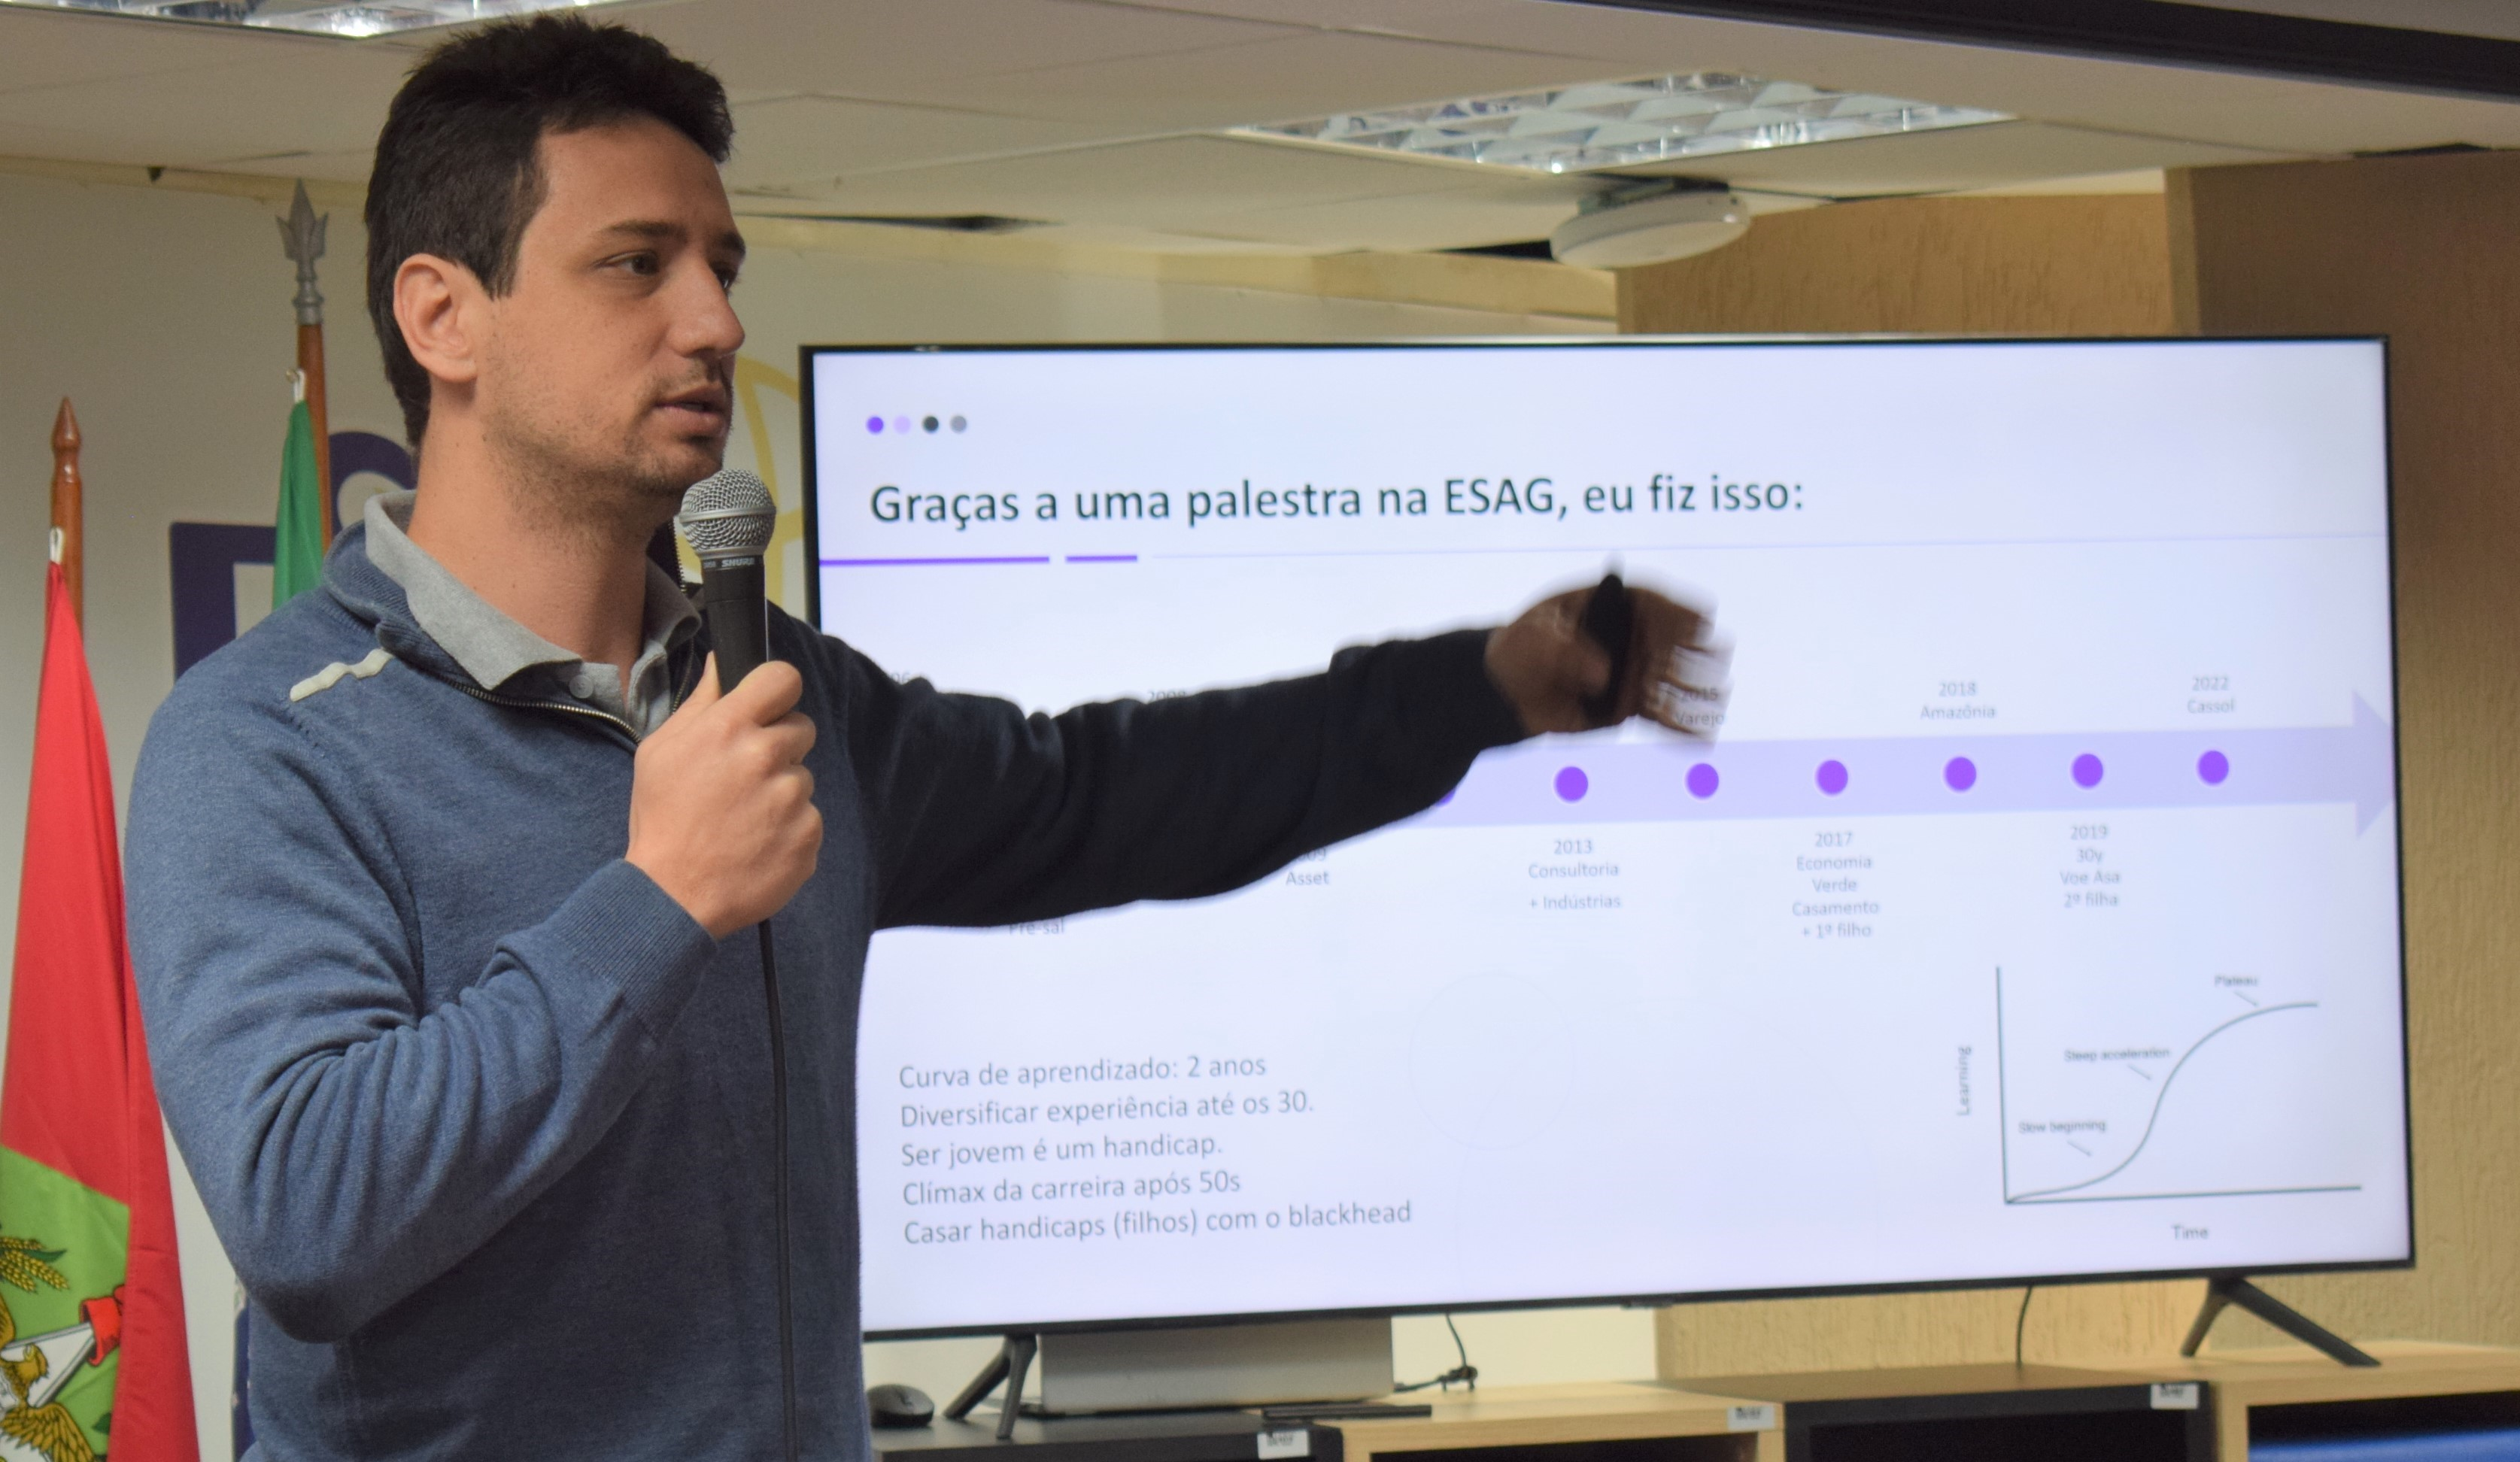
\includegraphics[width=0.8\textwidth]{img/exemplo_img.jpg} % Substitua "img/exemplo_img.jpg" pelo caminho correto do arquivo de imagem
        % De preferência, use imagens com resolução alta para evitar distorções e dentro da pasta "img" para manter organização
        \caption{Figura Exemplo: Imagem de Palestra} % Legenda ou descrição adicional para explicar a imagem
    \end{figure}
    
    % Legenda ou descrição adicional para explicar a imagem
    \textbf{Descrição da Imagem:}
    Essa imagem ilustra uma palestra sobre ambientalismo econômico.
    \newline
    \newline % Use \newline para adicionar uma quebra de linha e não bater no final do slide
\end{frame}

% Slide com conteúdo adicional a imagem e com referências

\begin{frame}
    % Slide com conteúdo adicional a imagem e com referências
    \textbf{Referências:}
    \begin{itemize}
        \item \cite{udesc} - Notícia sobre palestra de ambientalismo econômico da UDESC.
    \end{itemize}
    % Use este espaço para adicionar mais referências ou conteúdo adicional
\end{frame}

\begin{frame}
    \textbf{Conteúdo Adicional:}
    \begin{itemize}
        \item Sempre cite as fontes e referências utilizadas.
        \item Caso seu slide não tenha nenhuma referência, você tem de comentar a linha \texttt{\texttt{\textbackslash bibliographystyle\{abntex2-alf\}}} e \texttt{\texttt{\textbackslash bibliography\{References\}}} no arquivo \texttt{main.tex}.
    \end{itemize}
\end{frame} % Está dando o erro "LaTeX Font: Font shape `OMS/lmtt/m/n' undefined (Font)	using `OMS/cmsy/m/n' instead (Font)	for symbol `textbackslash'." Pode ignorar esse erro, pois ele não afeta a compilação do documento e ele só acontece por usar o comando \ textbackslash que é só um exemplo de uso de comandos LaTeX. 


% O conteúdo dos slides é inserido no arquivo "content.tex" na pasta "textual". Foi definido um arquivo separado para facilitar a organização e edição do conteúdo. Caso deseje adicionar mais arquivos de conteúdo para melhor organização, basta cria-los na pasta "textual" e incluí-los aqui com o comando \include{textual/seuarquivo.tex} (substitua "seuarquivo" pelo nome do arquivo).

% Adicione mais slides conforme necessário, seguindo a estrutura dos slides de exemplo fornecidos no arquivo "content.tex".

% Slide de Referências
% As referências são inseridas no arquivo "References.bib" e são exibidas automaticamente no slide de referências ao final da apresentação. Caso não deseje exibir as referências, comente as linhas \bibliographystyle{abntex2-alf} e \bibliography{References} no final do arquivo e não use o comando \cite{} no conteúdo dos slides.

\bibliographystyle{abntex2-alf}
\bibliography{References}

\end{document} % Fim do documento
